% !TeX root = ../main.tex
% Add the above to each chapter to make compiling the PDF easier in some editors.

\chapter{Related Work}\label{chapter:relatedWork}
In this chapter, we give an overview about the existing work in the domain of the visualization of database performance profiling.
We will investigate the importance of optimizing query executions in database systems and the role of visualizations in identifying potential improvements.
As performant measurement and analysis play a crucial role in developing and optimizing database systems, 
it is essential to examine the state-of-the-art techniques and tools that have been used in this domain.
We will also cover a visualization tool closely associated with this thesis, as its key feature is integrated into the Benchy Viewer.



\section{Database Performance Profiling }

Performance profiling in database systems is crucial for optimizing their execution regarding achieving optimal hardware utilization and query efficiency.
Profiling the performance of database systems involves collecting and analyzing various performance metrics during query execution.
\\Besides profilers presenting results at the instruction and function granularity, a paper on "Profiling Dataflow Systems on Multiple Abstraction Levels" \cite{profiling-dataflow} proposes a solution that tracks the code generation process and aggregates profiling data to higher abstraction levels. This approach helps bridging the semantic gap between low-level profiles and high-level constructs, making it easier for developers to interpret profiling results and identify bottlenecks and hotspots in the system. The paper introduces the concept of Tailored Profiling, which extends the compilation steps to annotate the generated code with metadata. This enables the mapping of profiling results back to desired abstraction levels and provides more understandable profiling data.
Building on the insights from this work, the opportunity arises to create more meaningful visualizations regarding the dataflow in system performance profiling.
\\ An essential concept of this thesis is to build upon the concepts of tailored profiling to gain a deeper understanding of the system's performance and support the location of potential optimization possibilities. Thus, we integrate an intuitive and interactive query plan visualization feature that is able to break down complex queries into their constituent operators and pipelines. We clarify further details about the query plan in section \ref{subsec:semantic-diff} and in chapter X (Implementation) \textcolor{red}{Todo: Chapter linking}.

\section{Related visualization tools}

This section explores related visualization tools that aid developers analyse their database system queries, with a specific focus on performance visualization. We will go through the Query Plan Difference Visualizer and the Umbra Profiler \textcolor{red}{Todo: Zitat}, which are both tools, that are strongly related to the Benchy Viewer. 


\subsection{Query Plan Difference Visualizer}
\label{subsec:semantic-diff}

The Query Plan Difference Visualizer is a web application that compares and visualizes physical query execution plans from different relational database systems, as shown in Figure~\ref{fig:semantic-diff}.
\begin{figure}[h]
    \centering
    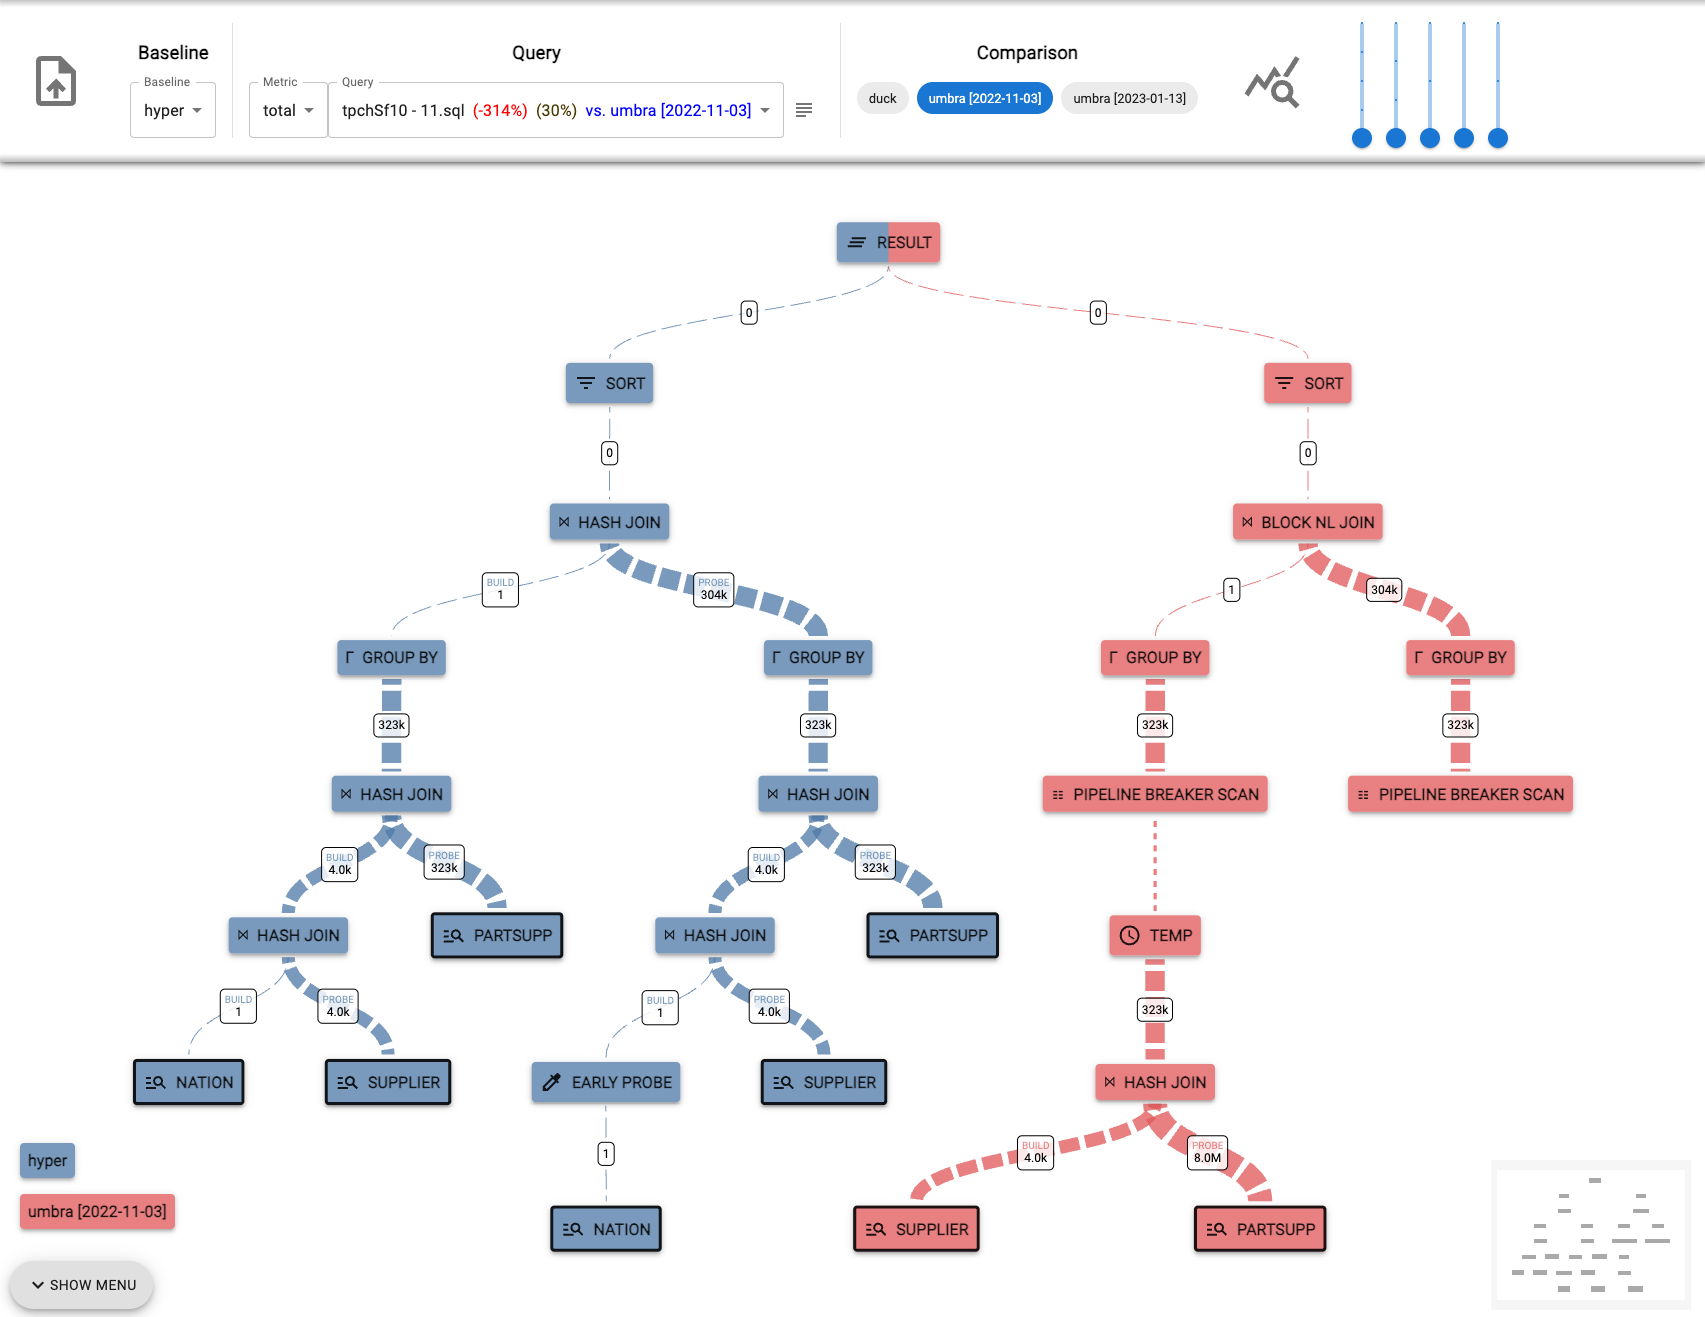
\includegraphics[width=0.8\linewidth]{figures/semantic-diff.png}
    \caption{Query Plan Difference Visualizer}
    \label{fig:semantic-diff}
  \end{figure}

\noindent The comparative tool is designed for database developers who want to inspect the correlation between variations in query execution speed and the respective query plans. Through enhanced hierarchical differencing algorithms with semantic information about query plans, the tool is able to interactively capture and present  the difference between query plans.
\\This is particularly useful for comparing different database systems or different versions of the same system, when varying query plans are used by the systems under test to process the same query.
\\This tool is strongly related to this thesis, since the Benchy Viewer builds upon the Query Plan Difference Visualizer by integrating its core features and providing the ability to compare query plans. We will dive deeper into the integration in Chapter X. \textcolor{red}{Todo: Chapter linking}



\subsection{Umbra Profiler}
The Umbra Profiler is a tool that enables an in-depth analysis for identifying bottlenecks in query execution processes of the database system Umbra.
\\ It is integrated with a backend application for preparing extensive profiling data and offers multiple perspectives, including a runtime dashboard, memory dashboard and an instruction dashboard, each depicting distinct information, as illustrated in Figure~\ref{fig:umbra-profiler}.
\textcolor{red}{Wie detailliert soll ich auf Funktionen vom Umbra Profiler eingehen? Z.B welche Diagramme es gibt und welche Metriken sie darstellen? }
\begin{figure}[h]
    \centering
    
\includegraphics[width=1\linewidth]{figures/umbra-profiler.png}
    \caption{Umbra-Profiler: Tool for analyzing and profiling Umbra’s compiling queries. From left-to-right: Runtime dashboard, memory dashboard, and instruction dashboard.}
    \label{fig:umbra-profiler}
  \end{figure}

\noindent Similar to the Benchy Viewer, the goal is to support database engineers in optimizing query execution by providing an interactive user interface, enabling an effective in-depth analysis process. 
\\The Umbra Profiler is designed based on the innovative Tailored Profiling approach \cite{profiling-dataflow}, where the connection between query plans and compiled code is maintained. This technique was previously unadressed by standard profilers and is now used in both the Umbra Profiler and the Benchy Viewer.  
\textcolor{red}{Mehr drauf eingehen, was es beim Benchy Viewer nicht gibt?}.
\\However, unlike the Benchy Viewer, the Umbra Profiler is focused to operate exclusively with the database system Umbra. In contrast, the Benchy Viewer has the versatility to function with multiple database systems or multiple instances of a single database system.
\\In broad terms, the Umbra Profiler is primarily designed for in-depth analysis of query performance within a single database system, while the Benchy Viewer is oriented towards its comparative function, enabling the comparison of queries executed by different instances. This comparative approach is the main essence  of the concept of the Benchy Viewer, which aims to enhance the understanding of differences between database instances.



